\documentclass[10pt,twocolumn,letterpaper]{article}

\usepackage{cvpr}
\usepackage{times}
\usepackage{epsfig}
\usepackage{graphicx}
\usepackage{amsmath}
\usepackage{amssymb}

% Include other packages here, before hyperref.

% If you comment hyperref and then uncomment it, you should delete
% egpaper.aux before re-running latex.  (Or just hit 'q' on the first latex
% run, let it finish, and you should be clear).
\usepackage[breaklinks=true,bookmarks=false]{hyperref}

\cvprfinalcopy % *** Uncomment this line for the final submission

\def\cvprPaperID{****} % *** Enter the CVPR Paper ID here
\def\httilde{\mbox{\tt\raisebox{-.5ex}{\symbol{126}}}}

% Pages are numbered in submission mode, and unnumbered in camera-ready
%\ifcvprfinal\pagestyle{empty}\fi
\setcounter{page}{4321}
\begin{document}

%%%%%%%%% TITLE
\title{Progress report: Anomaly detection in image data sets using deep learning}

\author{Kumar Saketh, Ali Radha\\
Department of EECS\\
University of Michigan\\
{\tt\small \{ksreddy,aliradha\}@umich.edu}
% For a paper whose authors are all at the same institution,
% omit the following lines up until the closing ``}''.
% Additional authors and addresses can be added with ``\and'',
% just like the second author.
% To save space, use either the email address or home page, not both
}

\maketitle
%\thispagestyle{empty}

%%%%%%%%% BODY TEXT
\section{Overview of work done}
Thus far, we have worked on identifying anomalies in the MNIST data set. To identify anomalies, we have implemented the current state-of-the-art method based on reconstruction errors described in \cite{h2o}. We have also implemented our proposed approach of building an unsupervised auto-encoder on the MNIST images, and then using the features learned by the auto encoder as input to the $k$-nearest neighbor (kNN) anomaly detection algorithm [please see section 5 of ~\cite{adsurvey}] and the Isolation Forest~\cite{iforest} anomaly detection algorithm in order to detect anomalies (please see Section 2.1 of the project proposal for details).

\section{Reading progress}
In order to implement the work described in the overview, we had to learn about three new methods - (1) auto-encoders, (2) kNN anomaly detection algorithm and (3) isolation forest algorithm. We learned about (1) from the UFLDL tutorial by Andrew Ng~\cite{ufldl}, about (2) from the survey paper \cite{adsurvey} and about (3) from the original paper on Isolation Forests~\cite{iforest}.

\section{Implementation progress}
By following the tutorial instructions in \cite{ufldl}, we successfully implemented a single hidden layer auto-encoder (illustrated in Figure~\ref{autoencoder}) in Matlab. This auto encoder learns features by minimizing reconstruction error between the input, and the output composed of the learned features. The input and output nudes of this network are equal to the number of pixels in each MNIST image = 28*28. We chose the number of nodes in the hidden layer to be 50 based on work done in \cite{h2o}. After training the auto-encoder network, we used the network to represent each MNIST image as a 50-dimensional vector corresponding to the 50 nodes in the hidden layer. We use the following notation in the sequel. Denote the MNIST image collection by ${\cal{I}}$ comprising of $n$ images ${\cal{I}} = \{I_1, I_2, \dots, I_n\}$. Denote the corresponding 50-dimensional feature representation of each image by ${\cal{F}} = \{F_1, F_2, \dots\, F_n\}$, with each $F_j \in \mathbb{R}^{50}$.

\begin{figure}[ht!]
\centering
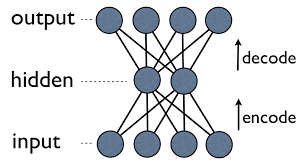
\includegraphics[width=50mm]{figs/autoencoder.png}
\caption{Illustration of autoencoder.}
\label{autoencoder}
\end{figure}

\subsection{Reconstruction error based method} We used the 50 dimensional vector $F_j$ corresponding  to each image $I_j$ in order to reconstruct the image using the learned auto-encoder. Denote the corresponding reconstructed output image as $O_j$. Then, for each image, we determine the normalized reconstruction error as $R_j = ||I_j - O_j||_2/||I_j||_2$. Then we determine the anomalous images by ordering images in decreasing order of reconstruction error and selecting the top images wrt this list.

\subsection{Feature based method}  We feed the feature set $ {\cal{F}} $ through two anomaly detection methods. First, we implemented the kNN algorithm, which determines anomalies by computing the average distance of each image $I_j$ to its $k=30$ nearest neighbors with respect to the feature set ${\cal{F}}$, and then ordering images in descending order of largest average nearest neighbor distance. 

\begin{figure*}[ht!]
\centering
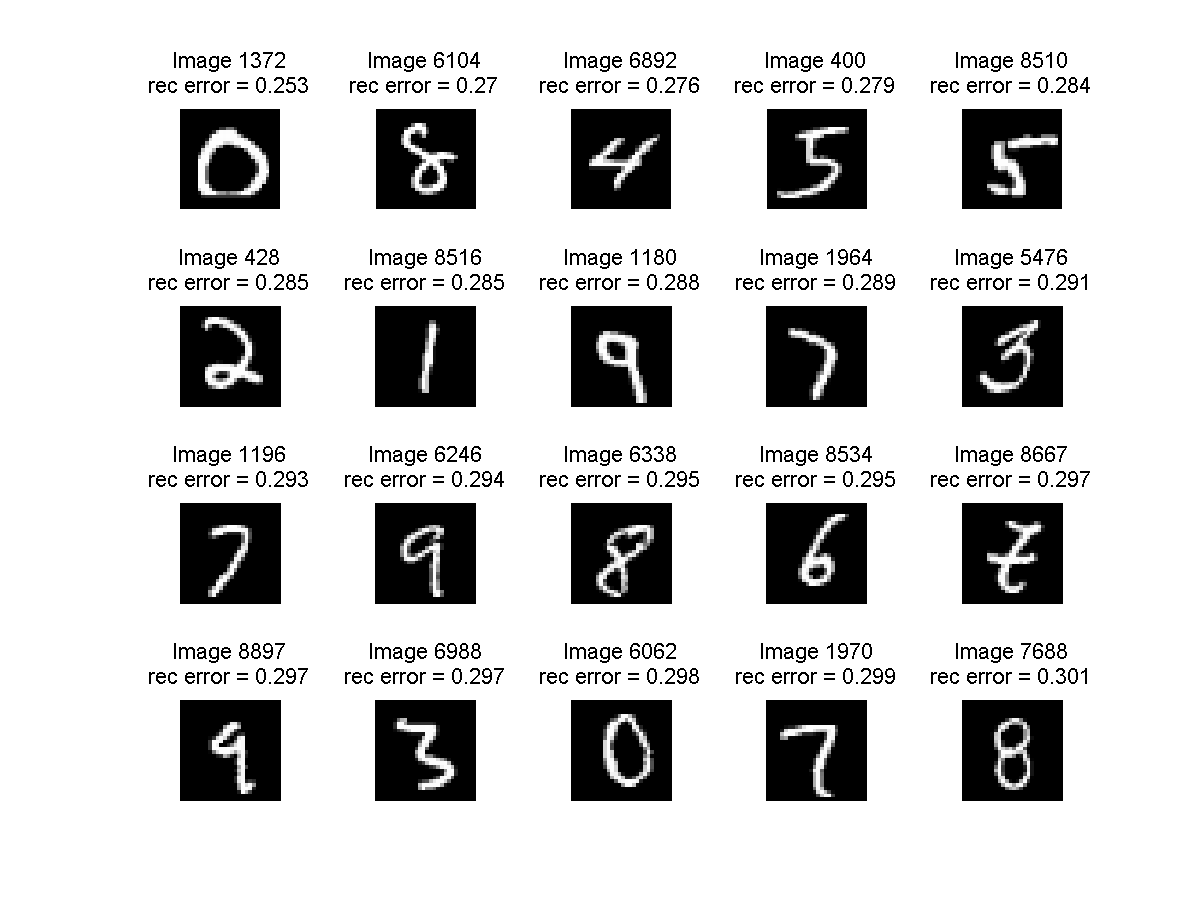
\includegraphics[width=60mm]{figs/normal.png}
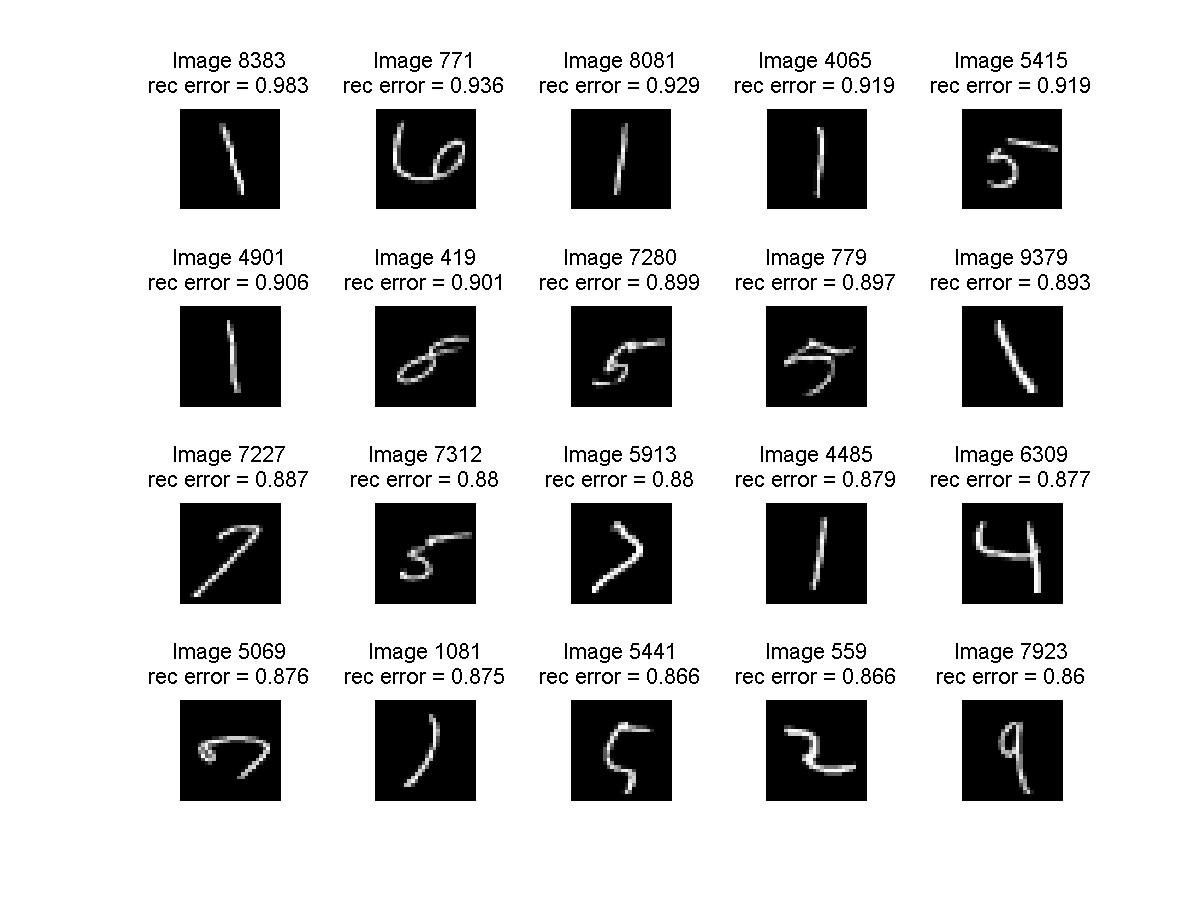
\includegraphics[width=60mm]{figs/top_rec_error.png}
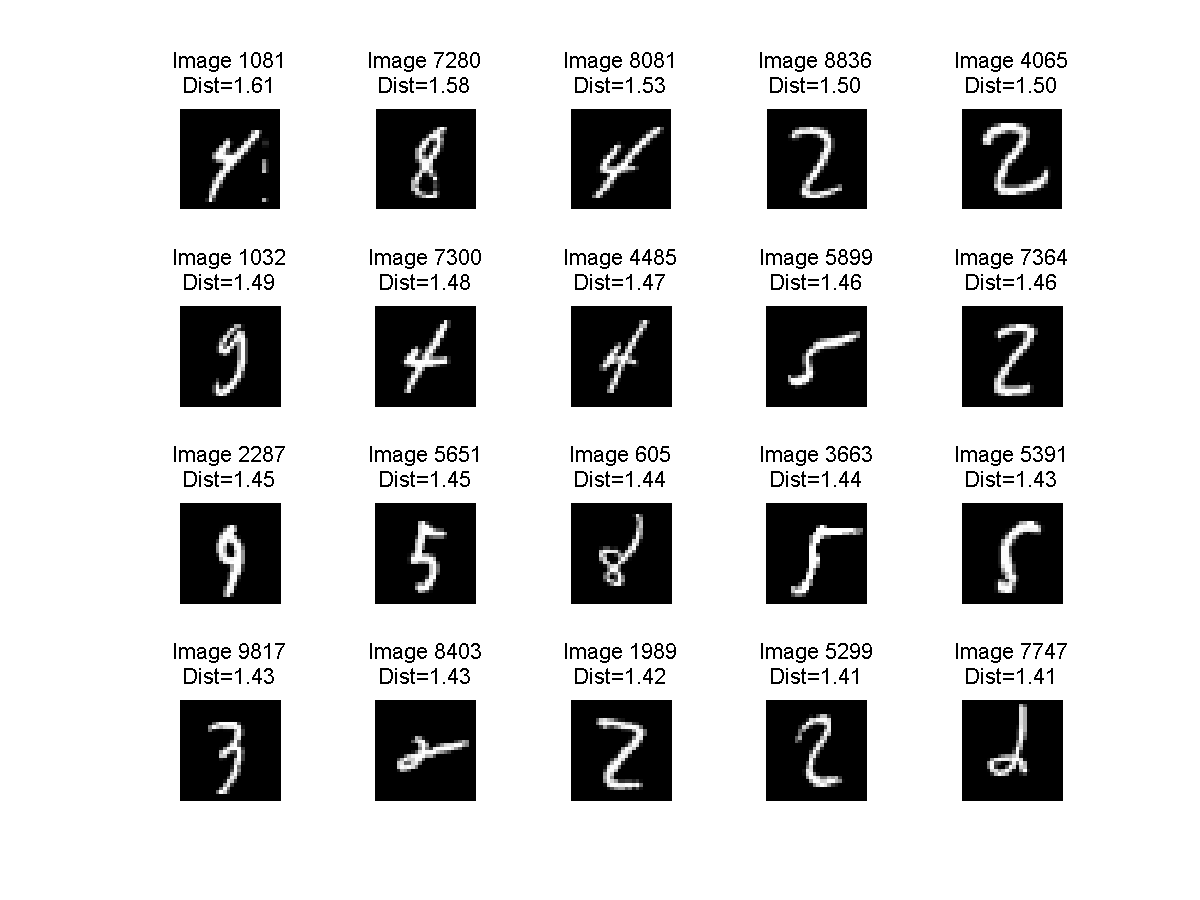
\includegraphics[width=60mm]{figs/top_dist.png}
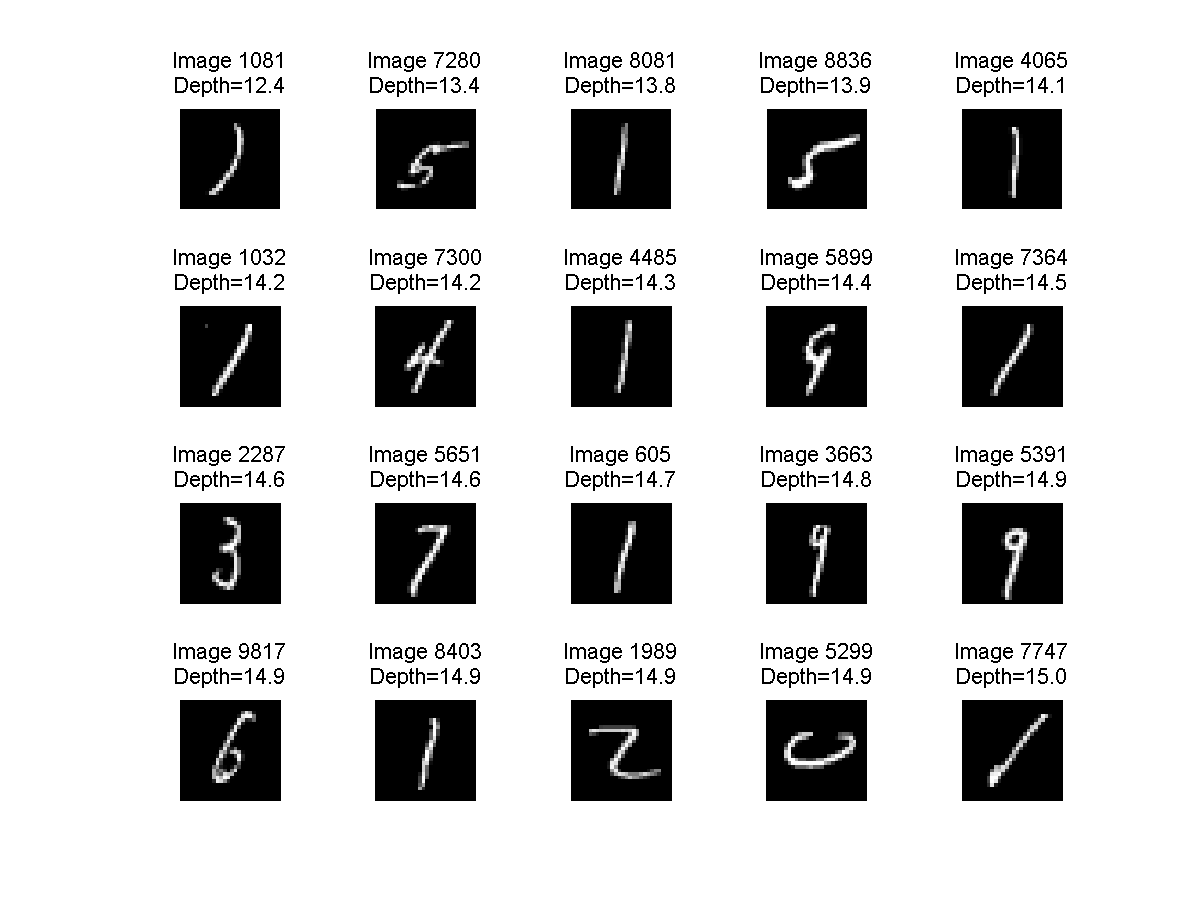
\includegraphics[width=60mm]{figs/iforest_error.png}
\caption{Four sets of MNIST images. Clockwise from top left: Normal images, anomalies wrt reconstruction error, Isolation forest, kNN.}\label{overflow}
\end{figure*}
We also implemented the Isolation Forest (iForest) algorithm in Python - the reason we chose Python was due to speed concerns. Our implementation involved the use of loops and we believed that Python was a better choice for this reason compared to Matlab. The iForest algorithm involves construction of isolation trees, which recursively partition the data by randomly splitting the data along a randomly chosen axis. The number of cuts needed to isolate a point is then used as an indicator of the anomalousness of the point - the more easy it is to isolate a point (i.e., smaller isolation depth in the tree), the more anomalous the point is. We computed a total of 2000 isolation trees and used the average isolation depth of each point as the measure of anomalousness.

\subsection{Comparison of results}
In the MNIST dataset, because we do not have labels on which points are normal and which are anomalous, we are currently restricted to qualitatively comparing the performance of these algorithms. In Figure~\ref{overflow}, we display the top 20 images for each of the following categories: (i) images with lowest reconstruction error, (ii) images with highest reconstruction error, (iii) images with smallest isolation depth, and (iv) images with highest kNN distance. 

Based on these results, we make the following observations: (i) the results of the kNN method seem to be qualitatively better than both the reconstruction method and the iForest method - in particular, the later two algorithms seems to be picking several '1' digits that look fairly normal to us; (ii) it also appears that the reconstruction error methods picks digits which are anomalous because of their orientation; (iii) the kNN methods picks digits which are anomalous because certain strokes are exaggerated in length (for e.g., see 4's in the kNN image set).   

\section{Todo}
(0) We would like to study the current results in further depth - in particular, to understand why the performance of iForest is relatively worse compared to kNN though both are operating on the same feature spaces. We would also like to understand if there is a fundamental difference in the type of anomalies being identified by the reconstruction method and the feature based methods.

(1) Next, we would like to implement a method to quantitatively compare the performance of our algorithms. We plan to do this by constructing anomaly detection data sets from classification data sets using the method described in ~\cite{benchmark}, and then using the Area under the ROC curve as a quantitative metric.

(2) We plan to run our algorithms on noisy image data sets like ImageNet in order to see if our proposed schemes are more robust in the presence of background noise relative to the reconstruction based method.  

(3) Finally, we would like to explore alternative neural network architectures including multi-layer autoencoders and deep belief nets.


\small{
\begin{thebibliography}{1}

\bibitem{adsurvey}
Chandola, Varun, Arindam Banerjee, and Vipin Kumar. "Anomaly detection: A survey." ACM Computing Surveys (CSUR) 41.3 (2009): 15.
\bibitem{h2o}
\url{http://learn.h2o.ai/content/hands-on_training/anomaly_detection.html}

\bibitem{iforest}
Liu, Fei Tony, Kai Ming Ting, and Zhi-Hua Zhou. "Isolation forest." Data Mining, 2008. ICDM'08. 

\bibitem{ufldl}
Ng, Andrew, et al. "UFLDL tutorial." (2012).

\bibitem{benchmark}
Emmott, A. F., Das, S., Dietterich, T. G., Fern, A., Wong, W.-K. (2013). "Systematic construction of anomaly detection benchmarks from real data". ODD '13 Proc. of ACM SIGKDD Workshop on Outlier Detection and Description.

\end{thebibliography}
}

\end{document}
